\section{Method}
\label{sec:method}
\begin{figure*}[t]
    \centering
    
\includegraphics[width=1\linewidth]{figures/pipeline.pdf}
    \vspace{-4mm}
    \caption{\textbf{Method Overview.} Our method stabilizes the scene geometry through three stages. In the static stage, we stabilize the geometry of the static scene by minimizing photometric loss $\mathcal{L}_{\text{color}}$ between vanilla 3DGS renders and ground truth images. The dynamic stage combines canonical 3D Gaussians $\textbf{G}$ with a deformable Gaussian MLP to model dynamic scenes while simultaneously minimizing normal loss $\mathcal{L}_{\text{normal}}$ between rendered normal map $\mathbf{N}^t$ and gradient normal map from depth map ${\mathbf{D}^t}$, thus further enhancing the overall scene geometry. Finally, the specular stage introduces a deformable reflection MLP to handle changing environment lighting, deforming reflection directions $\omega^t_r$ to query a canonical environment map for specular color $\mathbf{c}_s^t$. It is then combined with diffuse color $\mathbf{c_d}$ (using zero-order spherical harmonics) and learnable specular tint $\mathbf{s_\mathbf{tint}}$ per 3D Gaussian to obtain the final color $\mathbf{c}_\mathbf{final}^t$. This approach enables the modeling of dynamic specular scenes and high-quality novel view rendering.}
    \label{fig:pipeline}
\end{figure*}

\noindent {\bf Overview of the approach.}
The overview of our method is illustrated in Fig.  \ref{fig:pipeline}. Given an input monocular video sequence of frames and corresponding camera poses, we design a three-stage approach to reconstruct the dynamic specular scene, as detailed in Sec.~\ref{sec:Specular Rendering}. Accurate specular reflection requires precise normal estimation, so Sec.~\ref{sec:Normal Estimation} elaborates on how we estimate normals in dynamic scenes. Finally, we introduce the losses used throughout the training process in Sec.~\ref{sec:losses}.





\subsection{Preliminary} \label{sec:Deformation 3D Gaussians}


\vspace{3pt}  \noindent {\bf 3D Gaussian Splatting.}
Each 3D Gaussian is defined by a center position $\bm{x} \in \mathbb{R}^3$ and a covariance matrix $\bm{\Sigma}$. 3D Gaussian Splatting~\citep{kerbl20233d} optimizes the covariance matrix using scaling factors $\bm{s} \in \mathbb{R}^3$ and rotation unit quaternion $\bm{r} \in \mathbb{R}^4$. For novel-view rendering, 3D Gaussians are projected onto 2D camera planes using differentiable splatting~\citep{yifan2019differentiable}:
\begin{equation}
\mathbf{\Sigma}^{\prime}\mathbf{=}\mathbf{J}\mathbf{W}\mathbf{\Sigma}\mathbf{W}^{T}\mathbf{J}^{T}.
\end{equation}
Pixel colors are computed using point-based volumetric rendering:
\begin{equation}
C = \sum_{i \in {N}} {T}_i \mathbf{\alpha}_i {c}_i, \quad \mathbf{\alpha}_i = \mathbf{\sigma}_i e^{-\frac{1}{2} (\bm{x})^T \mathbf{\Sigma}' (\bm{x})},
\end{equation}
where ${T}_i = \prod_{j=1}^{i-1} (1 - \alpha_j)$ is the transmittance, $\sigma_i$ is the opacity, and $\mathbf{c}_i$ is the color of each 3D Gaussian.


\subsection{Specular Rendering}
\label{sec:Specular Rendering}
Since accurate reflections depend heavily on precise geometry, we implement a three-stage coarse-to-fine training strategy: static, dynamic, and specular stages. This approach ensures both stable scene geometry and accurate specular rendering.
% \paragraph{Limitations of existing methods.}
% Current Dynamic 3DGS methods~\citep{wu20234d,yang2023deformable} struggle with specular objects due to low-order spherical harmonics' inability to capture high-frequency details like specular highlights. While some static scene 3DGS-based methods~\citep{jiang2023gaussianshader,liang2023gs} use environment maps to handle specular reflections, these approaches aren't suitable for dynamic scenes. This limitation makes existing 3DGS-based methods inadequate for modeling dynamic scenes with specular objects.


% \paragraph{Proposed solution overview.}
% To overcome these limitations, we propose  physical normal estimation (Sec. \ref{sec:Normal Estimation}) paired with deformable environment maps to model specular color in dynamic scenes. Since accurate reflections depend heavily on precise geometry, we implement a three-stage coarse-to-fine training strategy: static, dynamic, and specular stages. This approach ensures both stable scene geometry and accurate specular rendering.




\subsubsection{Coarse-to-Fine Training Strategy} \label{sec:coarse_to_fine}
\noindent {\bf Static stage.}
In the static stage, we employ vanilla 3DGS~\cite{kerbl20233d} for static scene reconstruction to stabilize the geometry of the static scene. Specifically, we optimize the position $\bm{x}$, scaling $\bm{s}$, rotation $\bm{r}$, opacity $\alpha$, and coefficients of spherical harmonics (SH) of the 3D Gaussians by minimizing the photometric loss $\mathcal{L}_{\text{color}}$ identical to 3DGS~\citep{kerbl20233d}.


\vspace{3pt}  \noindent {\bf Dynamic stage.}
Following the static stage, we address dynamic objects using Deformable 3DGS~\cite{yang2023deformable}. For each 3D Gaussian in canonical 3D Gaussians $\textbf{G}$, we input its position $\bm{x}$ and time $t$ into a deformable Gaussian MLP with parameters $\theta_{\textit{G}}$ to predict position, rotation, and scaling residuals: $(\Delta\bm{x}^t,\Delta\bm{r}^t,\Delta\bm{s}^t) = F_{\theta_G}(\gamma(x), \gamma(t))$, where $\gamma$ denotes positional encoding. 
Attributes of the corresponding 3D Gaussian in deformed 3D Gaussians $\textbf{G}^t$ at time $t$ is obtained by $(\bm{x}^t,\bm{r}^t,\bm{s}^t)=(\Delta\bm{x}^t,\Delta\bm{r}^t,\Delta\bm{s}^t) + (\bm{x},\bm{r},\bm{s}).$

This approach separates motion and geometric structural learning, allowing accurate simulation of dynamic behaviors while maintaining a stable geometric reference.
To further enhance scene geometry, we estimate normals of deformed 3D Gaussians and optimize them using: 
% $\mathcal{L}_{\text{normal}} = 1 - {\mathbf{N}^t}\cdot\hat{\mathbf{N}^t},$ 
\begin{equation}
\mathcal{L}_{\text{normal}} = 1 - {\mathbf{N}^t}\cdot\hat{\mathbf{N}^t},
\end{equation}
where ${\mathbf{N}^t}$ is the rendered normal map and $\hat{\mathbf{N}^t}$ is the normal map derived from the rendered depth map ${\mathbf{D}^t}$. This process improves local associations among 3D Gaussians and optimizes both depth and normal information across the entire scene.


\vspace{3pt}  \noindent {\bf Specular stage.}
We adopt an image-based lighting (IBL) model, where the
environment light is given by a learnable cubemap. Following the rendering equation~\citep{kajiya1986rendering}, split-sum approximation~\citep{karis2013real, Munkberg_2022_CVPR}, and Cook-Torrance reflectance model~\citep{cook1982reflectance}, the outgoing radiance of the specular component $L_s$ is expressed as:
\begin{align}
L_s = \int_{\Omega} & \frac{DGF}{4 (\omega^t_o \cdot \mathbf{n}^t) (\omega_i \cdot \mathbf{n}^t)} 
    (\omega_i \cdot \mathbf{n}^t) d\omega_i \notag \\
    & \times \int_{\Omega} L_i(\omega_i) D(\omega_i, \omega^t_o) 
    (\omega_i \cdot \mathbf{n}^t) d\omega_i,
    \label{eq:specular_reflection}
\end{align}
where $\Omega$ is the hemisphere around the surface normal $\mathbf{n}^t$ (describe in Sec.~\ref{sec:Normal Estimation}.) $D$, $G$, and $F$ represent the GGX normal distribution function~\citep{walter2007microfacet}, geometric attenuation, and Fresnel term, respectively. $\omega^t_o$ is the view direction, and $L_i(\omega_i)$ is the incident radiance.
In the first term, we follow the GaussianShader ~\citep{jiang2024gaussianshader} directly computed by $\mathbf{s}_\text{tint} * F_1 + F_2$, where $F_1$ and $F_2$ are two pre-computed scalars depending on roughness $\rho$, view direction $\omega^t_o$ and normal $\mathbf{n}^t$. Roughness $\rho \in [0, 1]$ and specular tint $\mathbf{s_\mathbf{tint}} \in [0, 1]^3$ are learnable parameters for each 3D Gaussian. The second term is pre-integrated in a filtered learnable cubemap, where each mip-level corresponds to a specific roughness value. The cubemap can be queried using the reflection direction to obtain the value of the second term. After the static and dynamic stages, the geometry is well-defined. This allows us to calculate reflection directions $\omega^t_r = 2 (\omega^t_o \cdot \mathbf{n}^t) \mathbf{n}^t - \omega^t_o$ accurately.

$L_s$ represents only the specular color of the static environment light. To handle time-varying lighting in dynamic scenes, we introduce a deformable environment map, detailed in the following section.





\subsubsection{Deformable Environment Map for Dynamic Lighting.}

The concept of a deformable environment map involves treating the vanilla environment cubemap as a canonical environment map and combining it with a deformation field. This approach enables us to model time-varying lighting conditions effectively. We first apply positional encoding to the reflection direction $\omega^t_r$ and time $t$ to implement this. These encoded values are then input into a deformable reflection MLP with parameters $\theta_{\textit{R}}$. This process allows us to obtain the deformed reflection residual $\Delta\bar\omega^t_r=F_{\theta_{\textit{R}}}(\gamma(\omega^t_r),\gamma(t))$ for each specified time $t$.

Subsequently, we add the deformed reflection residual $\Delta\bar\omega^t_r$ to the reflection direction $\omega^t_r$, yielding the deformed reflection direction $\bar\omega^t_r=\Delta\bar\omega^t_r + \omega^t_r$.

We can then use this deformed reflection direction $\bar\omega^t_r$ to query the canonical environment map. The queried value is then multiplied by the first term of Equation \ref{eq:specular_reflection}, allowing us to obtain time-varying specular color $\mathbf{c}_s^t$. This approach effectively captures the dynamic nature of lighting in the scene while maintaining a stable canonical reference.


\subsubsection{Color Decomposition and Staged Training Strategy.}

We decompose the final color $\mathbf{c}_\mathbf{final}^t$ into diffuse and specular components to better distinguish between high and low-frequency information: $\mathbf{c}_\mathbf{final}^t = \mathbf{c}_d + \mathbf{c}_s^t$,
where $\mathbf{c_d}$ is the diffuse color (using zero-order spherical harmonics as view-independent color), and $\mathbf{c_s}^t$ is the view-dependent color component.
To manage the transition from spherical harmonics to $\mathbf{c}_\mathbf{final}^t$ and mitigate potential geometry disruptions, in the early specular stage, we fix the deformable Gaussian MLP and most 3D Gaussian attributes, optimizing only zero-order SH, specular tint, and roughness. We temporarily suspend densification during this phase. As $\mathbf{c}_\mathbf{final}^t$ becomes more complete, we gradually resume optimization of all parameters and reinstate the densification process.

We further split the specular stage into two parts, applying a coarse-to-fine strategy to the environment map. In the first part, we focus on optimizing the canonical environment map for time-invariant lighting. This establishes a stable foundation for the overall lighting structure. In the second part, we proceed to optimize the deformable reflection MLP for dynamic elements. This approach ensures a more robust learning process, allowing us to capture the static lighting conditions before introducing the complexities of dynamic components.




\begin{figure*}[t]
    \centering
    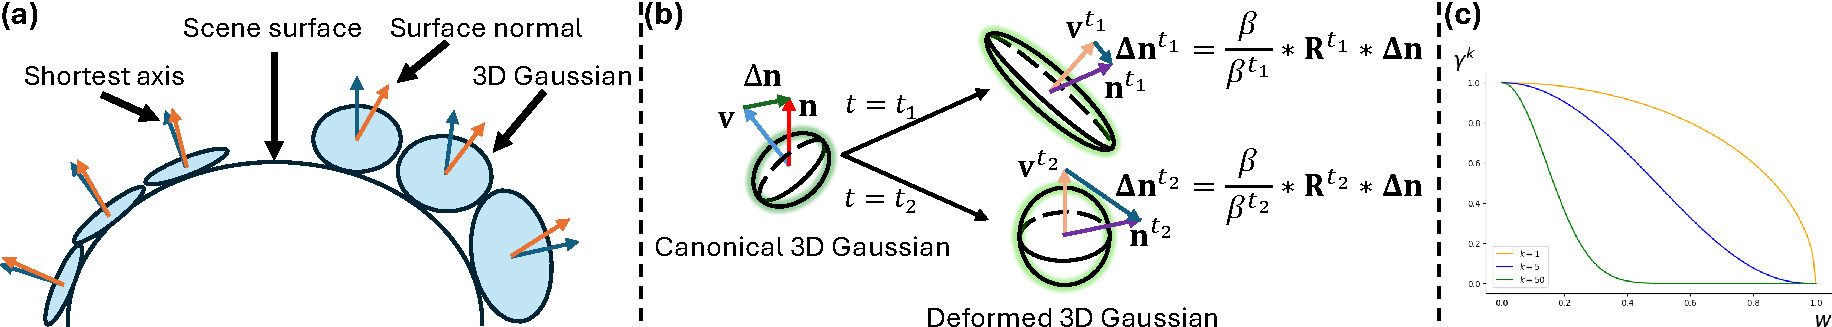
\includegraphics[width=1\linewidth]{figures/normal.pdf}
    \caption{\textbf{Normal estimation.} \textbf{(a)} shows that flatter 3D Gaussians align better with scene surfaces, their shortest axis closely matching the surface normal. In contrast, less flat 3D Gaussians fit less accurately, with their shortest axis diverging from the surface normal. \textbf{(b)} shows that when the deformed 3D Gaussian becomes flatter ($t=t_1$),  normal residual $\Delta\mathbf{n}$ is rotated by $\mathbf{R}^t_1$ and scaled down by $\frac{\beta}{\beta^t_1}$, as flatter Gaussians require smaller normal residuals. Conversely, when the deformation results in a less flat shape ($t=t_2$), $\Delta\mathbf{n}$ is rotated by $\mathbf{R}^t_2$ and amplified by $\frac{\beta}{\beta^t_2}$, requiring a larger correction to align the shortest axis with the surface normal. \textbf{(c)} shows how $\gamma^k$ changes with $w$ (where $w = \frac{|\mathbf{v}_s^t|}{|\mathbf{v}_l^t|}$) for $k=1$, $k=5$, and $k=50$. Larger $w$ indicates less flat Gaussians, while smaller $w$ represents flatter Gaussians. As $k$ increases, $\gamma^k$ decreases more steeply as $w$ rises. For $k=5$, we observe a balanced behavior: $\gamma^k$ approaches 1 for low $w$ and 0 for high $w$, providing a nuanced penalty adjustment across different Gaussian shapes.}
    \label{fig:normal_estimation}
\end{figure*}

\subsection{Physical Normal Estimation}
\label{sec:Normal Estimation}
\noindent {\bf Challenges in normal estimation for 3D Gaussians.}
Normal estimation is essential for modeling specular objects in 3D Gaussians, where GaussianShader \citep{jiang2023gaussianshader} initially used the shortest axis combined with a residual normal for approximation. While this works for static scenes, it becomes problematic with deformed Gaussians because the residual should vary at each time step. A straightforward approach of rotating the residual normal based on quaternion differences between canonical and deformed states proves insufficient, as it does not account for shape changes during deformation. When deformation alters the relative axis lengths, the shortest axis assumption breaks down. This highlights the need for a more comprehensive approach that considers both rotational and shape deformation effects to achieve accurate normal estimation for dynamic specular objects.

\vspace{3pt}  \noindent {\bf Improved rotation calculation for deformed 3D Gaussians.}
To overcome the limitations of naive methods and accurately model the normal of deformed 3D Gaussians, we propose using both the shortest and longest axes of canonical and deformed Gaussians to compute the rotation matrix. This approach accounts for both rotation and shape changes during deformation.
We first align the deformed Gaussian's axes with those of the canonical Gaussian using the following method:
\begin{align}
\mathbf{v}_s^t =
\begin{cases}
\mathbf{v}_s^t & \text{if } \mathbf{v}_s \cdot \mathbf{v}_s^t > 0, \\
-\mathbf{v}_s^t & \text{otherwise.}
\end{cases}
, \quad
\mathbf{v}_l^t =
\begin{cases}
\mathbf{v}_l^t & \text{if } \mathbf{v}_l \cdot \mathbf{v}_l^t > 0, \\
-\mathbf{v}_l^t & \text{otherwise.}
\end{cases},
\end{align}
where $\mathbf{v}_s$ and $\mathbf{v}_l$ represent the shortest and longest axes of canonical 3D Gaussians, while $\mathbf{v}_s^t$ and $\mathbf{v}_l^t$ denote the same for deformed 3D Gaussians. We then construct orthogonal matrices using these aligned axes and their cross-products:
\begin{equation}
\mathbf{U} = \begin{bmatrix} \mathbf{v}_s & \mathbf{v}_l & \mathbf{v}_s \times  \mathbf{v}_l \end{bmatrix},
\quad
\mathbf{V}^t = \begin{bmatrix} \mathbf{v}_s^t & \mathbf{v}_l^t & \mathbf{v}_s^t \times \mathbf{v}_l^t \end{bmatrix}.
\end{equation}
Finally, we derive the rotation matrix $\mathbf{R}^t = \mathbf{V}^t \mathbf{U}^\top.$

% This method provides a robust solution for calculating the rotation of deformation process, ensuring accurate normal estimation for dynamic specular objects.


\vspace{3pt}  \noindent {\bf Adjusting normal residuals and ensuring accuracy.}
To account for shape changes during deformation, we scale the normal residual based on the ratio of oblateness $\frac{\beta}{\beta^t}$ between canonical and deformed 3D Gaussians.
\begin{equation}
\beta = \frac{\lvert\mathbf{v}_l\rvert - \lvert\mathbf{v}_s\rvert}{\lvert\mathbf{v}_l\rvert},
\quad
\beta^t = \frac{\lvert\mathbf{v}_l^t\rvert - \lvert\mathbf{v}_s^t\rvert}{\lvert\mathbf{v}_l^t\rvert},
\end{equation}
where $\beta$ and $\beta^t$ represent the oblateness of canonical and deformed 3D Gaussians, respectively. This is because flatter 3D Gaussians tend to align more closely with the surface, meaning their shortest axis becomes more aligned with the surface normal, as shown in Fig. \ref{fig:normal_estimation} \textbf{(a)}. In such cases, less compensation from the normal residual is needed. Conversely, less flat Gaussians require more compensation, as illustrated in Fig. \ref{fig:normal_estimation} \textbf{(b)}. We then obtain deformed normal residuals:
\begin{equation}
\Delta\mathbf{n}^t = \frac{\beta}{\beta^t}\mathbf{R}^t\Delta\mathbf{n}.
\end{equation}
The final normal $\mathbf{n}^t$ is computed by adding this residual to the shortest axis and ensuring outward orientation:
\begin{equation}
\mathbf{n}^t = \Delta\mathbf{n}^t + \mathbf{v}_s^t,
\quad
\mathbf{n}^t =
\begin{cases}
\mathbf{n}^t &  \text{if } \mathbf{n}^t \cdot \omega^t_o > 0, \\
-\mathbf{n}^t & \text{otherwise.}
\end{cases}
\end{equation}
This approach adjusts for Gaussian flatness and ensures accurate normal estimation.


\subsection{Loss Functions} \label{sec:losses}
\noindent {\bf Normal regularization.}
To allow the normal residual to correct the normal while not excessively influencing the optimization of the shortest axis towards the surface normal, we introduce a penalty term for the normal residual:
\begin{equation}
\mathcal{L}_{\text{reg}} = \gamma^k\| \Delta \mathbf{n} \|_2^2
\quad
\text{where}
\quad
\gamma=\sqrt{1 - \frac{\lvert\mathbf{v}_s^t\rvert^2}{\lvert\mathbf{v}_l^t\rvert^2}}.
\end{equation}
In our experiments, we set $k = 5$. When $k=5$, less flatter 3D Gaussians have $\gamma^k$ approaching 0. Their shortest axis aligns poorly with the surface normal, requiring more normal residual correction and smaller penalties. Conversely, flatter Gaussians have $\gamma^k$ near 1. Their shortest axis aligns better with the surface normal, needing less normal residual correction and allowing larger penalties, as shown in Fig. \ref{fig:normal_estimation} \textbf{(c)}.



\vspace{3pt}  \noindent {\bf Total training loss.}
To refine all parameters in the dynamic and specular stages, we employ the total training loss:
\begin{equation}
\mathcal{L}=  \mathcal{L}_{\text{color}} + \lambda_{\text{normal}}\mathcal{L}_{\text{normal}} + \mathcal{L}_{\text{reg}},
\end{equation}
where $\mathcal{L}_{\text{color}}$ and $\mathcal{L}_{\text{normal}}$ are obtained as described in Section \ref{sec:coarse_to_fine}. 
% where $\mathcal{L}_{\text{reg}}$ is obtained as described in Section \ref{sec:Normal Estimation}. 
In our experiments, we set $\lambda_{\text{normal}} = 0.01$. Due to space constraints, complete implementation details are provided in the supplementary materials.
